\lecture{Proxy}{proxy}
\lecturetitle{\insertlecture}{\course}

\frame{\maketitle}

\begin{frame}{\insertlecture}

Um \alert{proxy} atua como intermediário entre o cliente e outro servidores
no atendimento às requisições de serviços em uma rede de computadores.

\pause
\begingroup
{\bf Proxy aberto}\bigskip

O \alert{proxy aberto} permite que qualquer usuário da internet faça
requisições de serviços na internet tendo o proxy como intermediário.

\begin{figure}
\centering
\includegraphics<2>[scale=.6]{proxy-open.png}

\caption{\footnotesize Proxy aberto. (Adaptado de 
\url{https://commons.wikimedia.org/wiki/File:Open_proxy_h2g2bob.svg})}
\end{figure}
\endgroup

\end{frame}

\begin{frame}{Proxy reverso}

O \alert{proxy reverso} atua como intermediário nas requisições de uma rede
interna e a internet. As requisições podem ser atendidas por um ou
mais proxies. Ele permite que haja um controle do tráfego de rede,
filtrando os recursos que podem ser acessados.

\begin{figure}
    \centering
    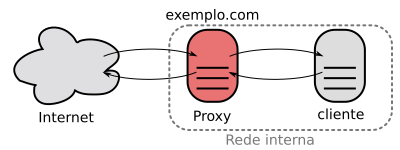
\includegraphics[scale=.6]{proxy-reverse.png}
    \caption{\footnotesize Proxy reverso. 
(Adaptado de 
\url{https://commons.wikimedia.org/wiki/File:Reverse_proxy_h2g2bob.svg})}
\end{figure}

\end{frame}

\begin{frame}{Serviços}{Proxy}

O usos mais comuns de proxy são:

\begin{description}
\item[Monitoramento e controle]: o proxy permite controlar o que pode
    entrar na rede interna, permitindo a criação de listas de sites
    que podem ser acessados, por exemplo.

\item[Melhoria da performance da rede]: o resultado das requisições
    pode ser armazenado em cache, fazem com que novas requisições do
    mesmo recurso sejam atendidas pelo proxy evitando que haja acesso
    a internet, economizando trafego na rede externa.

\item[Segurança]: um {\it firewall\/} pode ser configurado no proxy de modo que
a rede interna não sofra ataques comuns em hosts com acesso à
internet.
\end{description}

\end{frame}

\begin{frame}[fragile]{Serviços e ferramentas}


    \begin{itemize}
\item {DNS} ({\it Domain Name Service\/}):
\href{https://thekelleys.org.uk/dnsmasq/doc.html}{dnsmasq},
\href{https://www.isc.org/bind/}{BIND};

\item \href{https://pt.wikipedia.org/wiki/Dynamic_Host_Configuration_Protocol}{DHCP}:
\href{https://thekelleys.org.uk/dnsmasq/doc.html}{dnsmasq},
\href{https://www.isc.org/dhcp/}{ISC DHCP};

 \item \href{https://pt.wikipedia.org/wiki/Firewall}{Firewall}: \href{https://netfilter.org/}{iptables}, 
    \href{https://docs.freebsd.org/en/books/handbook/firewalls/}{PF}~(Package Filter);

\item \href{https://pt.wikipedia.org/wiki/Preboot_Execution_Environment}{PXE}
({\it Preboot Execution Environment\/}):
\href{https://thekelleys.org.uk/dnsmasq/doc.html}{dnsmasq},
\href{https://netboot.xyz/}{netboot.xyz};

\item \href{https://pt.wikipedia.org/wiki/BOOTP}{BOOTP}: 
\href{https://thekelleys.org.uk/dnsmasq/doc.html}{dnsmasq},
\href{https://www.ibm.com/docs/en/aix/7.2?topic=b-bootpd-daemon}{bootpd}.
\end{itemize}

\end{frame}

\begin{frame}{Ferramentas}{Proxy}

Uma ferramenta muito utilizada para a implantação de proxies é o
\href{http://www.squid-cache.org/}{Squid}.

\end{frame}